\chapter{Signes des fermions et annulations supersymétriques}

\lectureoverview{La supersymétrie relie bosons et fermions, mais on comprend mieux pourquoi on souhaite une telle relation avant d’en écrire l’algèbre. Nous partons de la topologie des rotations, rendons observable par interférence le signe de la fonction d’onde d’un fermion, déduisons le signe négatif d’une boucle fermionique fermée de l’antisymétrie par échange, puis utilisons les signes opposés des boucles bosoniques et fermioniques pour motiver l’annulation de l’énergie du vide et de l’auto-énergie des scalaires. Dans la seconde moitié, nous nous demandons dans quelle mesure la supersymétrie peut être brisée, comment détecter les partenaires supersymétriques et pourquoi une supersymétrie exacte ferait disparaître la structure ordinaire des couches atomiques.}

\section{Avant la supersymétrie : une particularité des rotations}

La supersymétrie est une symétrie entre fermions et bosons. Toutefois, avant d’essayer de la construire, il est utile de rappeler à quel point ces deux types de particules réagissent différemment aux rotations. Cette question commence par un fait topologique facile à démontrer, mais étonnamment difficile à oublier une fois qu’on l’a vu.

Tenez une main, paume tournée vers le haut, et faites pivoter le poignet de \(2\pi\). La main retrouve son orientation initiale, mais le bras, à l’évidence, n’est pas revenu à une configuration équivalente : il est vrillé. Continuez sur encore \(2\pi\), en faisant bouger le bras au besoin, et la torsion peut être défaite. Ainsi, une rotation de \(2\pi\) ne peut pas être déformée continûment en l’absence de rotation si l’on maintient l’environnement fixe, tandis qu’une rotation de \(4\pi\) le peut. La démonstration avec la main est une preuve par un geste de la main, au sens le plus littéral du terme.

On peut établir le même point sans s’appuyer sur l’anatomie. Placez une balle dans une boîte fixe et reliez-la aux parois par autant de ficelles flexibles et extensibles, mais incassables, que vous le souhaitez. Faites tourner la balle d’un tour de \(2\pi\). Les ficelles s’emmêlent, et aucun mouvement des ficelles seul ne permet de retrouver la configuration initiale. Faites tourner la balle d’un angle total \(4\pi\), et les ficelles peuvent être déplacées autour d’elle jusqu’à ce que l’entrelacs disparaisse. Les parois représentent l’infini spatial : la comparaison n’a de sens que parce que la frontière ne tourne pas avec la balle.

\begin{classroomqa}
\audiencequestion{Peut-on défaire l’entrelacs en faisant tourner la boîte ? \lecturetimestamp{00:02:53}}
\lecturerresponse{Cela change le problème. La boîte représente l’infini spatial et reste fixe. Nous comparons la rotation de l’objet par rapport à son environnement, et non une rotation commune de l’objet et de son environnement.}
\end{classroomqa}

\begin{classroomqa}
\audiencequestion{Pourquoi ne pas simplement faire tourner la balle d’un autre \(2\pi\)? \lecturetimestamp{00:03:20}}
\lecturerresponse{C’est précisément ce qui distingue les deux cas. Sans faire tourner davantage la balle, l’entrelacs laissé par un tour de \(2\pi\) ne peut pas être défait. Après un second tour, soit un total de \(4\pi\), il peut l’être.}
\end{classroomqa}

Dans le langage moderne des groupes, le groupe des rotations possède deux classes topologiques de chemins fermés :
\begin{equation}
\pi_1\!\left(SO(3)\right)\cong \mathbb Z_2.
\end{equation}
Un parcours unique est non trivial, tandis que deux parcours donnent la classe triviale.
De manière équivalente, \(SU(2)\) est le revêtement double de \(SO(3)\). C’est le
précédent géométrique du signe des fermions.

\editorialnote{\(SO(3)\), \(SU(2)\) et le langage du groupe fondamental explicitent la topologie. Les démonstrations avec le bras et avec les ficelles établissent géométriquement le même comportement à deux valeurs.}

\section{Ce qu’une rotation de \texorpdfstring{\(2\pi\)}{2 pi} fait à un état quantique}

Fixons maintenant la position d’une particule et ne retenons que son état de spin, noté \(\ket{\psi}\). Les particules de spin entier sont des bosons, et celles de spin demi-entier des fermions. On peut réaliser une rotation physique en plaçant un spin chargé dans un champ magnétique intense puis en faisant tourner le champ, ou en laissant le spin précesser de l’angle voulu dans un champ fixe.

\begin{classroomqa}
\audiencequestion{Comment peut-on réellement faire tourner le spin d’un électron en laboratoire ? \lecturetimestamp{00:05:26}}
\lecturerresponse{Un champ magnétique fournit le moyen d’agir sur le spin. On peut faire tourner un champ suffisamment intense pour que le spin le suive, ou laisser le spin précesser autour d’un champ fixe. Saisir l’électron à la main n’est pas une méthode expérimentale compétitive.}
\end{classroomqa}

Supposons qu’une rotation complète de \(2\pi\) multiplie l’état par une phase :
\begin{equation}
R(2\pi)\ket{\psi}=\xi\ket{\psi}.
\end{equation}
Effectuer l’opération deux fois donne
\begin{equation}
R(4\pi)\ket{\psi}=\xi^2\ket{\psi}.
\end{equation}
Comme le chemin de \(4\pi\) est topologiquement trivial, il doit agir comme l’identité dans cette comparaison. Par conséquent,
\begin{equation}
\xi^2=1,
\qquad
\xi=+1\ \hbox{or}\ -1.
\end{equation}
Les bosons correspondent au signe positif et les fermions au signe négatif :
\begin{align}
R(2\pi)\ket{\psi_B}&=+\ket{\psi_B},\\
R(2\pi)\ket{\psi_F}&=-\ket{\psi_F}.
\end{align}
Pour un état de spin bien défini \(j\), on peut résumer le résultat ainsi :
\begin{equation}
R(2\pi)=(-1)^{2j}.
\end{equation}
La transcription indique brièvement que la seconde possibilité correspond à une multiplication par \(2\pi\) ; la dérivation qui l’entoure et l’argument au tableau montrent clairement que le facteur attendu est \(-1\).

À première vue, cela semble dépourvu de conséquence physique. Si toute une fonction d’onde change de signe,
\begin{equation}
\Psi\longmapsto-\Psi,
\end{equation}
alors les probabilités restent inchangées, puisque
\begin{equation}
(-\Psi)^*(-\Psi)=\Psi^*\Psi.
\end{equation}
Considérons deux ensembles d’électrons préparés de façon identique. Faisons tourner chaque électron du premier ensemble de \(2\pi\) et laissons l’autre ensemble intact. Aucune mesure effectuée sur un électron isolé ne permet de savoir de quel ensemble il provient. Une phase globale n’est pas observable.

\section{Rendre le signe négatif relatif}

Le signe devient observable lorsqu’il est appliqué à une branche cohérente de la fonction d’onde, mais pas à l’autre. Envoyons des électrons un à un dans un dispositif à deux chemins. Ne déterminons pas le chemin emprunté, car l’information sur le chemin détruit les interférences. Notons les amplitudes des chemins supérieur et inférieur \(\psi_1\) et \(\psi_2\) ; l’état après recombinaison est alors
\begin{equation}
\Psi=\psi_1+\psi_2.
\end{equation}
Imaginons, provisoirement, que chaque branche soit piégée dans une région magnétique. Faisons tourner de \(2\pi\) le champ associé à la seconde branche seulement. Si la particule est un fermion, l’état devient
\begin{equation}
\Psi'=\psi_1-\psi_2.
\end{equation}
Il ne s’agit plus d’un signe global. La phase relative transforme les maxima d’interférence en minima. Si les deux paquets qui reviennent sont symétriques l’un de l’autre par rapport au centre du détecteur, la combinaison antisymétrique s’annule en ce point :
\begin{equation}
\Psi'(0)=\psi_1(0)-\psi_2(0)=0.
\end{equation}
L’électron n’est donc jamais détecté en ce point de symétrie. Faire tourner les deux branches produirait plutôt \(-\psi_1-\psi_2=-\Psi\), sans effet observable.

Le cours souligne le caractère relationnel de l’expérience. Faire tourner une région magnétique par rapport à l’autre revient à faire tourner la balle en maintenant la boîte fixe. Faire tourner les deux régions ensemble revient à faire tourner ensemble la balle et la boîte. Une rotation relative de \(4\pi\) annule l’effet, car l’état fermionique revient alors avec un signe positif. L’expérience a été proposée par Yakir Aharonov et Leonard Susskind en 1967, puis réalisée sous forme interférométrique, comme le signale incidemment le cours. Le même principe peut s’appliquer à des électrons ou à des ions chargés : le déplacement des franges identifie un état de spin demi-entier, tandis qu’un motif inchangé identifie un état de spin entier.

\begin{classroomqa}
\audiencequestion{Si l’on fait tourner le champ relatif de \(4\pi\), le motif déplacé revient-il à son état initial ? \lecturetimestamp{00:12:21}}
\lecturerresponse{Oui. Les deux changements de signe se multiplient pour donner \(+1\) ; la phase relative responsable de l’échange des maxima et des minima disparaît donc.}
\end{classroomqa}

\begin{classroomqa}
\audiencequestion{Dans quelle mesure faut-il associer littéralement les ficelles dans la boîte à un fermion ? \lecturetimestamp{00:13:43}}
\lecturerresponse{Elles constituent un aide-mémoire topologique, et non des ficelles physiques attachées à un électron. Un boson se comporte comme si un tour de \(2\pi\) ne laissait aucun souvenir ; un fermion conserve précisément le souvenir du signe représenté par l’entrelacs non trivial.}
\end{classroomqa}

\begin{classroomqa}
\audiencequestion{Y a-t-il deux électrons dans les deux régions magnétiques, l’un soumis à une rotation et l’autre non ? \lecturetimestamp{00:14:29}}
\lecturerresponse{Non. Il n’y a qu’un seul électron en superposition spatiale cohérente. Il possède une amplitude de probabilité d’occuper chacune des branches, et le dispositif ne doit pas révéler laquelle il a occupée. Faire tourner une région modifie une amplitude par rapport à l’autre ; les faire tourner toutes les deux ne modifie que la phase commune.}
\end{classroomqa}

L’angle \(2\pi\) est particulier : l’orientation du spin revient à sa valeur initiale, tandis que le spineur acquiert un signe. Une rotation relative générique modifie également l’orientation du spin. Si les deux états de chemin reviennent avec des états de spin \(\ket{\chi_1}\) et \(\ket{\chi_2}\), le terme d’interférence est proportionnel à
\begin{equation}
\braket{\chi_1}{\chi_2}.
\end{equation}
Son module détermine la visibilité des franges.\editorialnote{La formule du recouvrement des états de spin complète de manière standard la discussion qualitative du cours sur la perte partielle ou totale des interférences.} Des états de spin orthogonaux fournissent une information parfaite sur le chemin et n’interfèrent pas.

\begin{classroomqa}
\audiencequestion{Que se passe-t-il si l’on mesure dans quelle région magnétique se trouvait l’électron ? \lecturetimestamp{00:18:03}}
\lecturerresponse{Le motif d’interférence est détruit. Toute trace qui permet de distinguer les deux chemins supprime l’addition cohérente de leurs amplitudes.}
\end{classroomqa}

\begin{classroomqa}
\audiencequestion{Si tous les spins commencent dans la même direction et que l’on mesure le spin final, l’opération \(2\pi\) elle-même modifie-t-elle cette direction ? \lecturetimestamp{00:18:17}}
\lecturerresponse{Non. Après \(2\pi\), la direction physique du spin est la même ; seule la branche fermionique a acquis un signe négatif. C’est pourquoi cette opération peut modifier les interférences sans laisser une orientation de spin différente qui servirait de marqueur de chemin.}
\end{classroomqa}

\begin{classroomqa}
\audiencequestion{Que se passe-t-il si le champ ne tourne que de \(\pi\), au lieu de \(2\pi\) ? \lecturetimestamp{00:18:43}}
\lecturerresponse{La direction du spin change alors. Une branche de spin orienté vers le haut et une branche de spin orienté vers le bas sont distinguables et ne peuvent pas interférer. Aux angles intermédiaires, la visibilité diminue continûment ; une rotation relative de \(180^\circ\) la détruit complètement.}
\end{classroomqa}

\section{Symétrie d’échange et signe d’une boucle fermée}

La discussion sur les rotations a isolé un signe négatif caractéristique des fermions. Un second signe, étroitement lié au premier, apparaît lorsqu’on échange des particules identiques. Pour une fonction d’onde à deux particules,
\begin{align}
P_{12}\Psi_B(1,2)&=+\Psi_B(1,2)=+\Psi_B(2,1),\\
P_{12}\Psi_F(1,2)&=-\Psi_F(1,2)=-\Psi_F(2,1).
\end{align}
Les états bosoniques sont symétriques et les états fermioniques antisymétriques.

\begin{figure}[htbp]\centering
\includegraphics[width=0.74\textwidth]{lecture_02_figure_02.png}\lectureframe{00:24:27}\caption{Argument d’échange exprimé en notation des états. Seule l’étiquette du ket est lisible avec certitude sur l’image ; les équations d’antisymétrie sont composées en texte et ne sont pas attribuées à la craie masquée.}\end{figure}

Nous pouvons maintenant déterminer le signe relatif d’une boucle fermée de particule sans calculer son intégrale. Considérons un diagramme de Feynman du vide sans jambes externes. On peut le représenter comme une particule parcourant une trajectoire fermée dans l’espace-temps, ou comme une paire particule-antiparticule créée puis annihilée. Un tel diagramme du vide contribue à l’amplitude du vide et donc à l’énergie du vide.

Partons de deux copies déconnectées de la boucle. Les diagrammes déconnectés se multiplient ; si une boucle a pour signe \(\sigma\), la paire a donc pour signe
\begin{equation}
\sigma^2=+1.
\end{equation}
Coupons les deux boucles à un même instant, par exemple \(t=0\). À cette tranche temporelle, il y a deux particules identiques. Si nous les reconnectons sans les échanger, nous retrouvons les deux boucles séparées. Si nous échangeons les deux particules avant de les reconnecter, la topologie donne une seule boucle. L’échange apporte un facteur \(+1\) pour les bosons et \(-1\) pour les fermions. Comme le signe initial, pour les deux boucles, était positif, les signes obtenus pour une seule boucle sont
\begin{equation}
\begin{aligned}
\operatorname{sign}(\text{closed boson loop})&=+1,\\
\operatorname{sign}(\text{closed fermion loop})&=-1.
\end{aligned}
\end{equation}
Plus généralement, un diagramme comportant \(L_F\) boucles fermioniques fermées indépendantes porte le facteur
\begin{equation}
(-1)^{L_F}.
\end{equation}
Le cours déduit délibérément cette règle de l’échange au lieu d’invoquer l’intégration de Grassmann. Cet argument élémentaire rend visible l’origine physique du signe.

\section{Signes opposés des boucles et énergie du vide}

Une boucle bosonique du vide contribue avec un signe, tandis qu’une boucle fermionique contribue avec le signe opposé. Cela est immédiatement évocateur, car la densité observée de l’énergie noire est extrêmement faible par rapport aux estimations naïves obtenues avec une coupure en théorie quantique des champs. Le cours cite l’écart notoire, de l’ordre de \(123\) ordres de grandeur. L’exposant précis dépend de l’échelle ultraviolette choisie ; le point essentiel reste l’énorme décalage.

La valeur d’une boucle dépend de bien d’autres choses que de la statistique : elle dépend de la masse, de la charge, de la multiplicité et des interactions. Pourtant, si un boson et un fermion ont les mêmes propriétés pertinentes, leurs contributions de même module peuvent s’annuler :
\begin{equation}
\begin{gathered}
m_B=m_F,\qquad q_B=q_F,\qquad g_B=g_F,\\
\Delta\rho_{\mathrm{vac}}^{(B)}
+\Delta\rho_{\mathrm{vac}}^{(F)}=0.
\end{gathered}
\end{equation}
Cette observation ne résout pas le problème de la constante cosmologique. Elle fournit seulement ce que les seules boucles bosoniques ordinaires ne pouvaient fournir : des contributions de signe opposé. Dans une théorie globale supersymétrique exactement non brisée, les annulations de l’énergie du vide peuvent effectivement être exactes, sous les hypothèses appropriées ; après brisure de la supersymétrie, la très petite valeur non nulle observée demeure inexpliquée.\editorialnote{Cette réserve distingue la motivation présentée dans le cours du problème, bien plus difficile, de la constante cosmologique.}

On sait déjà qu’un appariement exact ne décrit pas la nature. Si l’électron avait un partenaire de spin zéro possédant la même masse et la même charge électrique, l’annihilation électron-positron par l’intermédiaire d’un photon virtuel pourrait en produire une paire :
\begin{equation}
e^-e^+\longrightarrow\gamma^*
\longrightarrow\widetilde e^-\widetilde e^+.
\end{equation}
Un scalaire chargé dégénéré n’aurait pas échappé aux expériences ordinaires des collisionneurs. La réflexion entre bosons et fermions ne peut donc pas être une symétrie exacte du spectre observé. Il s’agit d’une réflexion entre types de particules, et non d’une réflexion dans l’espace physique.

\section{La cible plus immédiate : l’auto-énergie scalaire}

L’énergie du vide en fournit une première illustration, mais le principal sujet de préoccupation du cours est l’instabilité radiative des masses scalaires. Un scalaire dont la masse nue est nulle peut recevoir une correction quadratiquement sensible à la coupure. Schématiquement,
\begin{equation}
\Delta m_H^2\sim \frac{g_B^2}{16\pi^2}\Lambda^2
\end{equation}
une boucle bosonique produit cette correction. Les masses des fermions bénéficient d’une protection différente : lorsqu’un fermion sans masse possède une symétrie chirale exacte, les corrections radiatives ne peuvent pas engendrer de terme de masse additif. C’était l’argument fondé sur les composantes gauche et droite du cours précédent.

Imaginons maintenant une symétrie assez contraignante pour réunir un scalaire et un fermion dans un même multiplet et apparier leurs interactions. Une boucle fermionique apparaît alors avec le signe opposé :
\begin{equation}
\Delta m_H^2
\sim
\frac{g_B^2-g_F^2}{16\pi^2}\Lambda^2+\cdots .
\end{equation}
Si la supersymétrie impose \(g_B=g_F\) et des masses égales, les termes quadratiques s’annulent. La protection du fermion est ainsi transmise à son partenaire bosonique. Il ne s’agit pas d’une simple coïncidence numérique entre deux diagrammes : la symétrie doit imposer l’annulation à tous les ordres et pour toutes les interactions autorisées.

La comparaison étendue au tableau montre le cours passer de boucles isolées à des corrections de boucle appariées pour des particules en propagation.

\begin{figure}[htbp]
\centering
\includegraphics[width=0.79\textwidth]{lecture_02_figure_04.png}
\lectureframe{00:40:23}

\medskip
\begin{tikzpicture}[scale=0.9]
\draw (-4.2,0) circle (0.55);
\draw[dashed] (-2.4,0) circle (0.55);
\draw (0,0) -- (3.7,0);
\fill (1.85,0) circle (0.055);
\draw (1.85,0) -- (1.85,0.25);
\draw[dashed] (1.85,0.85) circle (0.6);
\end{tikzpicture}\caption{Comparaison, à l’échelle du tableau, des topologies de boucle ordinaires et de celles des partenaires. Le schéma composé conserve uniquement le contraste topologique visible ; il n’attribue pas d’étiquettes aux particules masquées.}\end{figure}

Après la pause, l’argument reprend par ce que le cours appelle l’image d’ordre zéro. Il ne s’agit pas d’un ordre en théorie des perturbations, mais de la description utile la plus sommaire :
\begin{quote}
À chaque particule correspond un partenaire supersymétrique de statistique opposée. Chaque fermion a un partenaire bosonique, et chaque boson un partenaire fermionique.
\end{quote}
Dans une théorie supersymétrique exacte, les partenaires seraient aussi dégénérés, c’est-à-dire de même masse. La nature ne présente pas une telle dégénérescence. Pourtant, si leurs masses sont inégales sans trop différer, l’annulation peut rester suffisamment efficace pour éviter une correction scalaire démesurée. Avec une brisure douce de la supersymétrie, l’échelle dangereuse est remplacée, schématiquement, par l’écart entre les masses des partenaires supersymétriques :
\begin{equation}
\Delta m_H^2\sim
\frac{g^2}{16\pi^2}\,\Delta m_{\mathrm{SUSY}}^2
\ln\!\frac{\Lambda^2}{\Delta m_{\mathrm{SUSY}}^2}
\end{equation}
à des coefficients dépendant du modèle près.\editorialnote{Cette formule exprime qualitativement l’idée du cours : un appariement imparfait des masses laisse une correction résiduelle déterminée par l’écart ; elle n’est pas recopiée du tableau.}

\section{Supersymétrie brisée et pari expérimental de 2010}

Aucun partenaire supersymétrique n’avait été observé lorsque ce cours a été enregistré en 2010. On en déduisait immédiatement que, s’ils existaient, les partenaires devaient être plus lourds que les particules connues et au-delà de la portée des machines précédentes. Les modèles supersymétriques distinguent également les particules dont les masses apparaissent uniquement après la brisure de la symétrie électrofaible des états autorisés à avoir des masses plus élevées qui préservent la symétrie. Le cours présente cela comme une explication possible du fait que la moitié visible du spectre supersymétrique puisse être légère, tandis que la moitié encore invisible serait plus lourde, tout en reconnaissant franchement qu’il s’agit d’une hypothèse audacieuse. Susskind dit s’attendre personnellement à ce que des partenaires supersymétriques soient détectés, puis précise aussitôt qu’il s’agit d’une conjecture, et non d’un résultat.

Le Grand collisionneur de hadrons occupait donc une place centrale dans les perspectives du cours. Il devait rechercher à la fois le boson de Higgs et les partenaires supersymétriques. Ces propos doivent être compris dans leur contexte de 2010 : le cours expose les paris expérimentaux formulés avant la découverte du Higgs et avant les résultats ultérieurs des recherches au LHC.

Pourquoi un partenaire supersymétrique motivé par le naturel ne serait-il pas à l’échelle de Planck ? Parce qu’il ne remplirait alors plus le rôle qui lui est assigné. Si les masses du boson et du fermion diffèrent énormément, leurs intégrales de boucle cessent de s’annuler au-dessus de la masse la plus faible. La correction scalaire résiduelle est alors déterminée approximativement par l’écart important plutôt que par l’échelle électrofaible. Une supersymétrie à une échelle arbitrairement lointaine reste une symétrie mathématique, mais elle ne fournit plus d’explication convaincante à un secteur de Higgs léger.

Le cours traduit cela par l’attente, à l’époque, que les écarts pertinents se situent à quelques centaines de GeV environ et soient donc à la portée du LHC. Cette estimation numérique est historique et dépend du modèle ; le raisonnement est plus important :
\begin{equation}
\begin{gathered}
\text{Higgs protection}\\
\Downarrow\\
\text{effective boson--fermion cancellation}\\
\Downarrow\\
\Delta m_{\mathrm{SUSY}}\ \text{not too large}.
\end{gathered}
\end{equation}

\begin{classroomqa}\audiencequestion{Les contributions fermioniques pourraient-elles simplement compenser globalement toutes les contributions bosoniques, sans partenaires associés un à un ? \lecturetimestamp{00:45:01}}\lecturerresponse{Elles pourraient se compenser numériquement, mais il s’agirait d’une annulation accidentelle, aussi finement ajustée que le problème initial. La proposition supersymétrique est plus forte : des postulats raisonnables imposent des contributions appariées, tandis que la supersymétrie brisée explique pourquoi les masses ne sont appariées qu’approximativement. L’énergie du vide en était l’illustration ; ici, la préoccupation immédiate est l’auto-énergie du Higgs.}
\end{classroomqa}

\begin{classroomqa}\audiencequestion{Qualifier d’artificielle une annulation globale suppose-t-il déjà une conception réductionniste de l’organisation de la théorie ? \lecturetimestamp{00:47:51}}\lecturerresponse{C’est une objection légitime. Personne ne possède de définition définitive du naturel, et la recherche revient en partie à tâtonner pour trouver une explication convaincante. La supersymétrie et sa brisure spontanée offrent des cadres mathématiques connus qui peuvent imposer la structure souhaitée. Les questions sans réponse sont de savoir si la nature utilise ce cadre et s’il est unique.}
\end{classroomqa}

\section{Production directe, effets virtuels et chaînes de désintégration}

Une particule lourde n’a pas besoin d’être produite sur couche de masse pour influencer une expérience. Elle peut apparaître virtuellement à l’intérieur d’une boucle et modifier légèrement une amplitude ordinaire de diffusion électron-positron. Les mesures électrofaibles de précision contraignent donc les partenaires supersymétriques même lorsque l’énergie dans le centre de masse est inférieure au seuil de production directe de la paire
\begin{equation}
\sqrt{s}<2m_{\widetilde p}.
\end{equation}
Selon l’évaluation de 2010 présentée dans le cours, les données de précision réduisaient déjà l’espace des paramètres supersymétriques, sans toutefois l’exclure.

\begin{classroomqa}\audiencequestion{Peut-on inférer indirectement l’existence de partenaires supersymétriques, comme on a auparavant contraint des particules lourdes à partir de taux de production mesurés avec précision avant de les observer directement ? \lecturetimestamp{00:49:01}}\lecturerresponse{Oui. Une boucle virtuelle de partenaire supersymétrique modifie légèrement une amplitude ordinaire ; la question relève donc de la phénoménologie électrofaible de haute précision plutôt que de la production directe. Un collisionneur électron-positron propre et suffisamment énergétique serait particulièrement utile. Les collisions de protons sont plus difficiles à interpréter, car le proton est un état composite de quarks et de gluons : en réalité, ce sont des constituants fluctuants que l’on fait entrer en collision, et non deux particules élémentaires dont les conditions initiales seraient connues avec précision.}
\end{classroomqa}

Un étudiant demande si l’on pourrait faire réagir les particules en sens inverse, en partant d’une abondance de superparticules. L’obstacle n’est pas l’invariance par renversement du temps, mais leur disponibilité. Il faut d’abord créer les partenaires supersymétriques lourds, et la plupart devraient se désintégrer rapidement en états plus légers.

\begin{classroomqa}\audiencequestion{Si un univers contenait de nombreuses superparticules, deux d’entre elles pourraient-elles entrer en collision et se transformer en particules ordinaires ? \lecturetimestamp{00:53:43}}\lecturerresponse{En principe, les réactions correspondantes possèdent des réactions inverses, mais les partenaires supersymétriques lourds ne devraient pas rester abondants à l’état libre. Ils se désintègrent vers des états de plus basse énergie ; une expérience doit donc d’abord fournir une énergie de collision suffisante pour les créer.}
\end{classroomqa}

Cela soulève la question de la matière noire. Dans de nombreux modèles supersymétriques, une règle de sélection discrète empêche le dernier partenaire supersymétrique d’une chaîne de désintégration de disparaître complètement. Tous les partenaires supersymétriques plus lourds se désintègrent alors en cascade vers le partenaire supersymétrique le plus léger, ou LSP. Si le LSP est électriquement neutre, il peut être stable et difficile à détecter, ce qui en fait un candidat possible pour la matière noire. La transcription parle une fois d’« énergie noire » dans cet échange, mais la question de l’auditoire et la description de la particule concernent sans ambiguïté la matière noire.

\begin{classroomqa}\audiencequestion{La désintégration rapide des partenaires supersymétriques est-elle incompatible avec l’hypothèse qu’un partenaire supersymétrique puisse constituer la matière noire ? \lecturetimestamp{00:54:53}}\lecturerresponse{Non. La plupart des partenaires supersymétriques peuvent se désintégrer tandis que le plus léger reste stable dans les modèles qui imposent la présence d’un partenaire supersymétrique au terme de chaque chaîne de désintégration. La charge électrique entraîne généralement d’autres difficultés phénoménologiques ; le LSP viable est donc probablement neutre. Il n’est pas indétectable en principe, mais il ne laisserait pas la trace d’ionisation évidente d’un sélectron chargé.}
\end{classroomqa}

\section{L’appariement concerne aussi les couplages}

L’appariement des masses ne suffit pas. Comparons une boucle du vide de l’électron à une boucle du sélectron. Leurs statistiques opposées fournissent des signes opposés, mais des modules égaux exigent des masses égales. Ajoutons maintenant deux photons externes. Les coefficients comportent aussi les couplages électriques ; l’annulation exige donc des charges égales :
\begin{equation}
\begin{gathered}
q_{\widetilde e}=q_e,\\
\mathcal A_{\mathrm{loop}}^{(e)}
+\mathcal A_{\mathrm{loop}}^{(\widetilde e)}=0,\\
\text{provided the full couplings match.}
\end{gathered}
\end{equation}
Tout écart laisse un terme divergent qui ne s’annule pas. La supersymétrie est précieuse parce qu’elle relie aussi les interactions, et pas seulement les noms et les spins.

\begin{figure}[H]
\centering
\includegraphics[width=0.66\textwidth]{lecture_02_figure_05.png}
\lectureframe{00:57:15}

\medskip
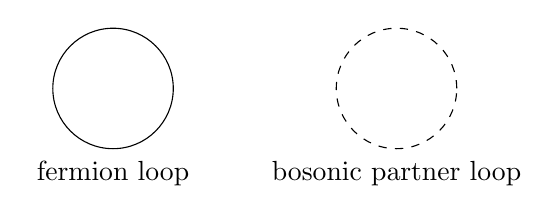
\begin{tikzpicture}[scale=0.9]
\draw (-2.0,0) circle (0.85);
\draw[dashed] (2.0,0) circle (0.85);
\node at (-2.0,-1.2) {fermion loop};
\node at (2.0,-1.2) {bosonic partner loop};
\end{tikzpicture}\caption{Comparaison des boucles pleines et pointillées au cours de l’argument sur l’appariement des charges. Les marques externes coupées ne sont pas reconstituées, car l’image seule ne permet pas de déterminer toutes les insertions.}\end{figure}

\begin{classroomqa}\audiencequestion{Les partenaires supersymétriques auraient-ils pu échapper à la détection simplement parce que leurs constantes de couplage sont différentes ? \lecturetimestamp{00:56:23}}\lecturerresponse{Pas si l’on veut que les mêmes diagrammes s’annulent. L’ajout d’interactions avec des photons permet de tester la charge électrique de chaque ligne. Des couplages inégaux donnent des facteurs de boucle numériques inégaux et rétablissent un grand terme résiduel. La symétrie doit apparier les charges et les interactions pertinentes.}
\end{classroomqa}

\begin{classroomqa}\audiencequestion{Le partenaire supersymétrique du photon devrait-il lui aussi être sans masse ? \lecturetimestamp{00:58:01}}\lecturerresponse{Il serait sans masse dans une théorie supersymétrique exacte, puisqu’il serait dégénéré avec le photon. Le monde observé n’étant pas exactement supersymétrique, un état physique de type photino n’a pas besoin d’avoir la même masse que le photon.}
\end{classroomqa}

\section{Le répertoire des partenaires supersymétriques}

Les règles de nomenclature ne sont pas élégantes, mais elles sont utiles. À un boson correspond un partenaire fermionique dont le nom se termine souvent par \emph{-ino} : photon et photino, \(W\) et wino, \(Z\) et zino, gluon et gluino, Higgs et higgsino, graviton et gravitino. À un fermion ordinaire correspond un partenaire bosonique dont le nom commence généralement par \emph{s-} : électron et sélectron, quark et squark.

\begin{center}
\begin{tabular}{@{}>{\raggedright\arraybackslash}p{0.40\linewidth}>{\raggedright\arraybackslash}p{0.52\linewidth}@{}}
\toprule
État ordinaire & superpartenaire et variation du spin\\
\midrule
Higgs scalaire, \(j=0\) & higgsino, \(j=\tfrac12\); \(\Delta j=+\tfrac12\)\\
boson de jauge, \(j=1\) & gaugino, \(j=\tfrac12\); \(\Delta j=-\tfrac12\)\\
fermion de matière, \(j=\tfrac12\) & sfermion, \(j=0\); \(\Delta j=-\tfrac12\)\\
graviton, \(j=2\) & gravitino, \(j=\tfrac32\); \(\Delta j=-\tfrac12\)\\
\bottomrule
\end{tabular}
\end{center}

La relation générale est que les membres d’un supermultiplet diffèrent d’une demi-unité de spin :
\begin{equation}
\Delta j=\frac12.
\end{equation}
Les exemples approximatifs donnés en cours associent un fermion de matière de spin-\(\tfrac12\) à un scalaire, et un boson de jauge de spin un à un gaugino de spin-\(\tfrac12\). Dans un modèle complet avec interactions, le mélange des états après la brisure de symétrie peut faire que les états propres de masse physique ne conservent pas ces noms élémentaires.

\begin{classroomqa}
\audiencequestion{Tous les nouveaux partenaires scalaires pourraient-ils subir leur propre brisure spontanée de symétrie ? \lecturetimestamp{01:01:27}}
\lecturerresponse{Les champs scalaires peuvent acquérir des valeurs moyennes, mais une brisure arbitraire de symétries supplémentaires aurait des conséquences phénoménologiques désastreuses. Un modèle supersymétrique viable doit organiser son potentiel scalaire de sorte que la couleur, la charge électrique et les autres symétries nécessaires ne soient pas brisées de manière inadéquate.}
\end{classroomqa}

\begin{classroomqa}
\audiencequestion{L’higgsino possède-t-il des interactions particulières correspondant au terme quartique du Higgs ? \lecturetimestamp{01:02:19}}
\lecturerresponse{La supersymétrie met en correspondance les interactions aussi bien que les particules. Cette relation ne s’obtient pas en remplaçant naïvement chaque ligne de Higgs par une ligne d’higgsino, mais le terme quartique scalaire et les interactions fermioniques et auxiliaires pertinentes relèvent d’une même structure contrainte. Ces détails n’ont pas encore été développés dans le cours.}
\end{classroomqa}

\begin{classroomqa}
\audiencequestion{Le théorème de rotation \(2\pi\) contre \(4\pi\) a-t-il des analogues dans d’autres dimensions ? \lecturetimestamp{01:03:07}}
\lecturerresponse{Oui, mais la dimension change les possibilités. Dans deux dimensions spatiales, les trajectoires d’échange peuvent s’enrouler les unes autour des autres, ce qui permet l’existence d’anyons dont les phases d’échange sont plus générales que celles des bosons, \(+1\), et des fermions, \(-1\). De telles excitations apparaissent dans des systèmes de matière condensée, mais elles ne font pas partie du parcours de ce cours.}
\end{classroomqa}

\section{Pourquoi une supersymétrie exacte ferait disparaître la chimie}

Nous nous demandons enfin à quoi ressemblerait un monde où la supersymétrie serait exacte. Ici, cela signifie que chaque paire particule-superpartenaire aurait des masses égales et des interactions correspondantes. L’électron aurait un sélectron bosonique de même masse et de même charge électrique, et le photon sans masse aurait un photino fermionique sans masse :
\begin{equation}
m_{\widetilde e}=m_e,
\qquad
q_{\widetilde e}=q_e,
\qquad
m_{\widetilde\gamma}=m_\gamma=0.
\end{equation}

La structure périodique bien connue de la chimie dépend de la statistique de Fermi. L’hydrogène possède un électron sur son orbitale la plus basse. L’hélium peut en accueillir deux sur cette orbitale, car leurs projections de spin diffèrent. Le troisième électron du lithium doit occuper une orbitale de plus haute énergie : le principe d’exclusion de Pauli empêche trois électrons identiques d’occuper le même état à une particule. Cet électron externe a une énergie plus élevée et préférerait tomber vers l’intérieur, ce qui émettrait normalement un photon, mais les états inférieurs déjà occupés bloquent la transition.

La supersymétrie exacte ouvre une autre voie :
\begin{equation}
e^-_{\mathrm{outer}}
\longrightarrow
\widetilde e^-_{\mathrm{inner}}
+
\widetilde\gamma .
\end{equation}
L’électron initial et le photino émis sont des fermions, tandis que le sélectron restant est un boson. Comme les sélectrons obéissent à la statistique de Bose plutôt qu’à celle de Fermi, rien n’interdit au sélectron final d’occuper une orbitale basse déjà occupée. L’électron de valence peut donc se convertir et tomber vers l’intérieur.

\begin{figure}[H]
\centering
\includegraphics[width=0.62\textwidth]{lecture_02_figure_06.png}
\lectureframe{01:09:18}

\medskip
\begin{tikzpicture}[scale=0.9]
\fill (0,0) circle (0.075);
\draw (0,0) circle (0.72);
\draw (0,0) circle (1.45);
\draw[-{Latex[length=2.2mm]}] (1.42,0.2) .. controls (1.2,0.52) and (0.92,0.42) .. (0.72,0.1);
\draw[decorate,decoration={snake,amplitude=1.4pt,segment length=7pt},-{Latex[length=2.2mm]}]
  (1.58,0) -- (3.55,0);
\node[above] at (2.7,0.12) {$\widetilde\gamma$};
\node[below] at (0,-1.65) {selectron drops to a lower orbital};
\end{tikzpicture}
La transition atomique qui illustre pourquoi la supersymétrie exacte changerait la chimie. La ligne ondulée sortante est visible ; son identification comme photino provient de la transcription.\caption{}
\end{figure}

Le phénomène ne se limite pas à un atome de type lithium. Dans un atome lourd, ce sont les électrons de valence qui créent la diversité chimique. S’ils peuvent se convertir à répétition en sélectrons bosoniques, ils peuvent se concentrer dans la région de plus basse énergie accessible au lieu de remplir des couches. Le résultat ressemblerait à une population bosonique concentrée près du noyau, et non à l’architecture familière des orbitales de valence. Les molécules formées de liaisons directionnelles et de couches partiellement remplies ne subsisteraient pas sous une forme reconnaissable. Le cours appelle \emph{slithium} le descendant hypothétique du lithium, mais la plaisanterie mène à une conclusion sérieuse : la supersymétrie exacte produirait une matière différente de la matière ordinaire, et donc une biologie différente de la biologie ordinaire.

\begin{classroomqa}
\audiencequestion{La transition de l’électron au sélectron pourrait-elle être si faiblement couplée que les atomes ordinaires survivraient ? \lecturetimestamp{01:10:23}}
\lecturerresponse{Pas dans la théorie exacte envisagée ici. La supersymétrie relie cette transition à l’interaction électromagnétique ; son couplage est donc fixé par la charge électrique et ne peut pas être choisi librement pour être infime. Le cours donne une durée de vie approximative de l’ordre de la microseconde pour un atome de type lithium, non comme résultat d’un calcul de précision, mais pour souligner que la désintégration serait rapide.}
\end{classroomqa}

Nous savons donc, à partir de la matière qui nous entoure et indépendamment des recherches menées auprès des collisionneurs, que la supersymétrie ne peut pas être exacte à basse énergie. L’écart entre les masses des particules et de leurs superpartenaires est immense à l’échelle atomique ou à celle du proton, même s’il serait infime à l’échelle de l’unification ou de Planck.

\begin{classroomqa}
\audiencequestion{Pourquoi, alors, la supersymétrie est-elle brisée ? \lecturetimestamp{01:11:19}}
\lecturerresponse{Le cours avance un argument de sélection minimal : si elle ne l’était pas, des observateurs constitués de matière régie par la chimie ordinaire ne seraient pas là pour poser la question. Cela ne remplace pas une théorie dynamique de la brisure de la supersymétrie. Cela explique seulement pourquoi un monde à supersymétrie exacte et à basse énergie ne pourrait pas être le nôtre.}
\end{classroomqa}

La brisure de la supersymétrie est mathématiquement possible et, dans de nombreuses constructions, plutôt générique, même si obtenir une brisure réaliste est loin d’être automatique. À l’inverse, les théories quantiques des champs à supersymétrie exacte possèdent une structure assez particulière pour que certaines puissent être étudiées bien plus en profondeur que les théories génériques. Elles servent à la fois de candidates pour organiser la physique des particules et de laboratoires mathématiques particulièrement puissants. Le cours suivant passera de cette motivation physique à l’étude d’une partie de cette structure.

\section{Le fil du raisonnement}

Le chemin qui mène à la supersymétrie a été délibérément indirect :
\begin{enumerate}
\item Une rotation spatiale de \(2\pi\) appartient à une classe topologique non triviale, tandis qu’une rotation de \(4\pi\) peut être déformée continûment jusqu’à l’identité.
\item Un état fermionique acquiert un signe moins sous \(2\pi\), et une expérience à deux chemins rend ce signe observable lorsqu’il est relatif plutôt que global.
\item L’antisymétrie des fermions par échange donne à chaque boucle fermionique fermée un signe moins supplémentaire par rapport à une boucle bosonique.
\item Les signes opposés des boucles permettent des annulations, imposées par la symétrie, des contributions du vide et de l’auto-énergie scalaire lorsque les masses et les couplages correspondent.
\item Dans la nature, cette correspondance exacte n’existe pas. Si la supersymétrie protège le secteur de Higgs, sa brisure ne peut pas rendre les superpartenaires pertinents arbitrairement lourds.
\item Une supersymétrie exacte à basse énergie permettrait aux électrons de se convertir en sélectrons bosoniques et ferait s’effondrer la structure en couches dont dépend la chimie ordinaire.
\end{enumerate}

La supersymétrie est donc séduisante et impossible sous sa forme naïve exacte pour la même raison : elle lie étroitement bosons et fermions. Cette relation étroite peut maîtriser les corrections quantiques dangereuses, mais si elle persistait sans être brisée jusqu’à l’échelle atomique, le monde cesserait de ressembler à celui qui nous entoure.